\documentclass[11pt]{article}
\usepackage[a4paper,margin=24mm]{geometry}
\usepackage[T1]{fontenc}
\usepackage[utf8]{inputenc}
\usepackage{lmodern,microtype}
\usepackage{amsmath,amssymb,amsthm,mathtools}
\usepackage{booktabs,longtable,array,tabularx}
\usepackage{enumitem,xcolor,graphicx,fancyhdr,needspace}
\usepackage[breaklinks=true,colorlinks=true,linkcolor=blue!45!black,
  citecolor=blue!45!black,urlcolor=blue!45!black]{hyperref}
\usepackage{listings}
\definecolor{ink}{HTML}{17384C}
\definecolor{pale}{HTML}{EEF4F7}
\hypersetup{pdftitle={Quadrilateral Support Kernels and Certified Normal-Disc Discovery},
  pdfauthor={Research continuation for the ProveIt project}}
\setlength{\parskip}{4pt}
\setlength{\parindent}{0pt}
\setlength{\headheight}{14pt}
\pagestyle{fancy}
\fancyhf{}
\fancyhead[L]{\small\textcolor{ink}{ProveIt / Unknot Recognition}}
\fancyhead[R]{\small 9 October 2026}
\fancyfoot[C]{\thepage}
\setlist{nosep,leftmargin=*}
\lstset{basicstyle=\ttfamily\footnotesize,breaklines=true,
  columns=fullflexible,keepspaces=true,backgroundcolor=\color{pale},
  frame=single,rulecolor=\color{pale},showstringspaces=false}
\newtheorem{theorem}{Theorem}[section]
\newtheorem{lemma}[theorem]{Lemma}
\newtheorem{proposition}[theorem]{Proposition}
\newtheorem{corollary}[theorem]{Corollary}
\theoremstyle{definition}
\newtheorem{definition}[theorem]{Definition}
\theoremstyle{remark}
\newtheorem{remark}[theorem]{Remark}
\newcommand{\R}{\mathbb R}
\newcommand{\Z}{\mathbb Z}
\newcommand{\Q}{\mathbb Q}
\newcommand{\F}{\mathbb F_2}
\newcommand{\poly}{\operatorname{poly}}
\newcommand{\supp}{\operatorname{supp}}
\newcommand{\rank}{\operatorname{rank}}
\newcommand{\diag}{\operatorname{diag}}
\newcommand{\norm}[1]{\left\lVert#1\right\rVert}
\newcommand{\code}[1]{\texttt{#1}}
\makeatletter
\renewcommand*\l@subsection{\@dottedtocline{2}{1.5em}{3.1em}}
\makeatother

\title{\textcolor{ink}{Quadrilateral Support Kernels and\\
Certified Normal-Disc Discovery}\\[5pt]
\large Exact cone reduction, support-dependent height bounds,\\
rank-sensitive search, and a barrier to uniform sparsity}
\author{Research continuation for Vladimir Reshetnikov's ProveIt project\\
\small Prepared with OpenAI ChatGPT; proofs, code, and independent audits included}
\date{9 October 2026}

\begin{document}
\maketitle
\begin{abstract}
The maintained unknot-recognition project now has compressed, independently
checked operations on a supplied normal surface, but finding a suitable surface
remains a separate task. We implement an exact discovery layer for a specified
compatible quadrilateral sector and derive explicit support-sensitive bounds.
If at most one quadrilateral type is allowed in each of $k$ tetrahedra, contracting
the triangle matching equations with identically zero quadrilateral contribution
reduces the standard normal cone, modulo independent vertex-link factors, to
at most $9k$ variables and $4k$ equations. The triangle block is a directed
incidence matrix and every quadrilateral column has $\ell_1$ norm at most four.
A determinant expansion therefore bounds every primitive standard vertex
triangle coordinate by $4^k$, and every positive quadrilateral coordinate by
$4^{k-1}$, independently of the total number $t$ of tetrahedra.

Two exact enumeration methods operate on this reduction: positive-support
enumeration in $2^{9k}\poly(t,k)$ time and a potential-arrangement method whose
number of linear systems depends on the quadrilateral matching nullity $d$.
Adapting the classical canonical Euler-characteristic convexity argument, a
preliminary Q-ray search tests only $\binom{k}{d-1}$ systems for $d>0$ to decide whether
the sector contains a canonical positive-Euler surface. Every positive disc
claim is checked by the existing weighted orbit machinery. Exhaustion has
explicitly restricted meanings.

The implementation agrees with independent Regina enumerations on 1,718
sectors in each phase, with 962 complete discovery-certificate replays and
60 rejected mutations. We also derive a limitation: the Fibonacci layered
solid tori force $\Omega(t)$ occupied quadrilateral tetrahedra for every
essential standard vertex disc. Sparse search is consequently a conditional
quasi-polynomial route, not a general solution. Dense sectors of nullity one
remain tractable and are included in the experiments. The package provides
proofs, portable Python code, exact fixtures, raw measurements, and integration
instructions. It does not establish a general quasi-polynomial unknot recognizer.
\end{abstract}

\clearpage
\tableofcontents
\newpage

\section{Outcome, source baseline, and relation to earlier work}
\label{sec:outcome}

\subsection{The concrete advance}

This continuation moves from evaluating a supplied normal vector to actually
constructing candidate vectors. The input is a finite triangulation $\mathcal T$
of a compact orientable three-manifold with one torus boundary, together with
allowed quadrilateral types. The output is either an independently checked
essential-disc witness or a precisely delimited statement about that sector.
An optional outer search enumerates small allowed supports.

The main mathematical refinement is the dependence on the number of allowed
quadrilateral types, rather than all standard coordinates. A triangulation may
contain many tetrahedra through which only triangles propagate. These tetrahedra
still have to be read and their geometric data retained, but they need not
contribute independent variables to the difficult cone search.

The three principal proved results are as follows.
\begin{enumerate}
\item An exact algebraic quotient of a compatible standard cone has at most
  $9k$ variables and $4k$ matching equations; an explicit integer-linear expansion
  reconstructs the original coordinates (Theorem~\ref{thm:kernel}).
\item Primitive standard vertex coordinates satisfy the sharper bounds
  $a_c\le4^k$ and $q_i\le4^{k-1}$, with a data-dependent product bound available
  (Theorem~\ref{thm:height}).
\item On Fibonacci layered solid tori, every essential standard vertex disc
  needs linear quadrilateral support (Theorem~\ref{thm:barrier}). This shows why
  the support bound alone cannot settle the general complexity objective.
\end{enumerate}
The exact search and certificate code make these statements executable.
The distinction between an algebraic candidate and an essential disc is
preserved throughout.

\subsection{Pinned repository state}

The source snapshot was read through the selected GitHub connection at
repository commit
\begin{quote}\small
\path{fdeb5b1a20b84b93cb150e0232031837bb7d30cb}.
\end{quote}
The latest relevant unknot commit in that snapshot is
\begin{quote}\small
\path{3a6c7e99fe0ea9fc37ab505d261e0d747acb8cf2}.
\end{quote}
The repository location is
\url{https://github.com/VladimirReshetnikov/ProveIt/tree/main/Topology/UnknotRecognition}.
The snapshot already includes sparse incidence, independently certified weighted
normal components, the quadrilateral disc-count core, and ordered compressed
group-certificate replay. The maintained synthesis describes these in
\path{synthesis/sparse_incidence.tex},
\path{synthesis/weighted_components.tex}, and the recent elimination sections.
The retrieved root README contains older historical test counts; the recent
modules and commit records are the appropriate baseline for this continuation.

We reuse the existing finite-manifold validator, integer coordinate encoding,
normal arc geometry, weighted orbit producer, and independent disc-count checker.
Two new modules are additive:
\begin{quote}\small
\path{fastunknot/normal_sector.py}\\
\path{fastunknot/normal_sector_verify.py}.
\end{quote}
No claim in this report depends on having rerun the entire historical
1,090-test suite. The reported validation is the new, specifically described
oracle and certificate audit. All bundled upstream runtime files are pinned
and unchanged; the integration patch adds only the new modules and tests.

\subsection{Attribution and the scope of originality}

Normal matching equations, the ambiguity of triangle coordinates up to vertex
links, canonical lifting, and the relationship between Q-vertices and standard
vertices are established theory. Tollefson's Q-theory supplies the foundational
coordinate reduction~\cite{tollefson}. Burton gives canonical extension and
conversion between quadrilateral and standard solution sets~\cite{burton2009};
in particular, his Corollary 4.4 and Lemma 4.5 give the canonical nature of
non-link standard vertices and the standard extremality of canonical Q-vertices.
Burton's quadrilateral--octagon paper explicitly uses potentials on the
vertex-link graph and proves the convexity of canonical Euler
characteristic~\cite[proofs of Theorems 4.5 and 5.5]{burton2010}.
Burton--Ozlen develop exact type search and rank-sensitive determinant
arithmetic~\cite{burtonozlen2013,burtonozlen2014}.

We therefore present the graph contraction, explicit $9k/4k$ bounds, incidence
minor refinement, and their executable combination as a support-sensitive
derivation and implementation for this project. We do not claim priority over
all literature for these numerical refinements. The standard ingredients and
the new derivations are identified individually rather than grouped under a
claim of a new general normal-surface theory.

\subsection{The quasi-polynomial target in the current literature}

Lackenby's 2021 lecture announces quasi-polynomial unknot recognition and
describes compressed hierarchies and accelerated hierarchy operations~\cite{slides}.
His July 2026 preprint proves a new hierarchy algorithm and develops useful
certificate machinery~\cite{lackenby2026}. Section 9 explicitly leaves some
steps without sufficiently detailed running-time estimates. Theorem 14.4
provides efficient compressed operations for a supplied normal surface; that
is different from an end-to-end bound on finding the required hierarchy.

The present work has the same important separation. An efficient fixed-sector
discovery operation is one algorithmic component. A quasi-polynomial bound for
all knot diagrams additionally needs control of sector selection, changes of
triangulation, peripheral provenance, and subsequent geometric operations.

\section{Coordinates, sectors, and the exact search contract}
\label{sec:contract}

\subsection{Finite triangulations and normal coordinates}

Let $\mathcal T$ have $t$ tetrahedra. Face identifications are affine maps encoded
by permutations of the four local vertices. We allow loops, multiple
identifications, repeated global vertices within one tetrahedron, and gluings
between two distinct faces of the same tetrahedron. Every unpaired face lies
in the boundary. The existing validator checks connectedness, orientability,
edge links, finite vertex links, and that the single boundary component is a
torus. Ideal vertices are outside this implementation's domain.

Write $a_{i,v}$ for the triangle coordinate at local vertex $v$ of tetrahedron
$i$, and $q_{i,j}$ for its three possible quadrilateral coordinates. An integral
vector is admissible when all coordinates are nonnegative, the face matching
equations hold, and at most one quadrilateral type is nonzero per tetrahedron.
The normal realization theorem identifies such vectors with embedded normal
surfaces up to normal isotopy~\cite[Theorem 5.1]{hlp}.

Each face matching equation compares the number of arcs cutting off one face
corner. In local notation it is
\begin{equation}
 a_c+q_{\alpha(e)}=a_d+q_{\beta(e)},
 \qquad a_d-a_c=b_e(q):=q_{\alpha(e)}-q_{\beta(e)}.
 \label{eq:difference}
\end{equation}
An absent or forbidden quadrilateral contributes zero. When the two displayed
quadrilaterals are the same variable, they cancel. This convention is essential
for self-gluings.

\begin{definition}[Allowed sector]
A sector $S$ selects one allowed quadrilateral type in each of $k$ distinct
tetrahedra and forces every other quadrilateral coordinate to zero. The $k$
selected coordinates remain nonnegative and are allowed to vanish. Denote the
resulting real standard-coordinate cone by $C_S$.
\end{definition}

Thus $k$ is an allowed-support size, whereas a particular candidate may have
smaller actual support. Since forbidden coordinates are fixed to zero,
$C_S$ is a face of the nonnegative matching cone. Its extreme rays are
therefore standard extreme rays of that cone. Every vector in $C_S$ satisfies
the quadrilateral compatibility condition.

\subsection{Vertex links and primitive rays}

For a global vertex $v$, let $L_v$ put one triangle at every local corner
representing $v$ and zero elsewhere. Its normal surface is a sphere for an
interior vertex and a disc for a boundary vertex. Therefore
\begin{equation}
 \chi(L_v)=2\quad\hbox{or}\quad1.
 \label{eq:linkchi}
\end{equation}
A primitive ray vector is a nonzero integral vector whose coordinate gcd is
one and which spans an extreme ray. Triangle-only rays are precisely
vertex links. They cannot be essential discs.

A primitive extreme-ray surface is connected. Indeed, if it were a disjoint
union, its component vectors would be nonzero integral vectors in the same
cone summing to the ray vector. Extremality makes every component a positive
scalar multiple of it. Primitivity forces an integral scalar: an integer
linear combination of its coordinates equals one, so any scalar producing
integral coordinates is itself integral. Two positive such scalars cannot
sum to one. This argument includes one-sided surfaces.

\subsection{Statements the interface is allowed to make}

Table~\ref{tab:statuses} fixes the semantics before any performance discussion.
An essential-disc witness concerns the supplied manifold; it becomes an unknot
certificate only when that manifold is independently bound to the input knot
exterior. The manifold validator checks its topology locally, but it does not
prove that correspondence.

\begin{table}[ht]
\centering\small
\begin{tabularx}{\textwidth}{@{}p{.34\textwidth}X@{}}
\toprule
Status & Exact meaning \\
\midrule
\code{DISC\_FOUND} & The supplied triangulation contains a verified essential
disc component in the returned normal vector. \\
\code{NO\_POSITIVE\_EULER} & The sector contains no canonical normal surface
with positive Euler characteristic. In particular it contains no essential
normal disc. \\
\code{POSITIVE\_EULER\_ONLY} & The complete Q-ray phase found positive Euler
characteristic, but none of its tested rays was an essential disc. \\
\code{NO\_VERTEX\_DISC\_IN\_SECTOR} & Complete standard-ray enumeration found
no essential standard vertex disc in this sector. \\
\code{NO\_VERTEX\_DISC\_UP\_TO\_SUPPORT} & The complete outer search found no
essential standard vertex disc using at most the requested support size. \\
\code{INCONCLUSIVE} & A configured allowance was exhausted; no exhaustion
certificate or negative conclusion is issued. \\
\bottomrule
\end{tabularx}
\caption{Search results are scoped to the supplied sector or triangulation.
None of these strings claims a correspondence with a knot diagram.}
\label{tab:statuses}
\end{table}

\section{An exact algebraic support kernel}
\label{sec:kernel}

\subsection{The triangle difference graph}

Construct a multigraph with one vertex for each of the $4t$ triangle
coordinates. Every face-corner matching equation gives an oriented edge from
$c$ to $d$, labelled by the integer linear form $b_e$ in
\eqref{eq:difference}. Reversing the orientation negates the form. The graph's
connected components are exactly the global vertex classes, since both
equivalence relations are generated by the same face-corner identifications.

Restrict all labels to the allowed variables in $S$. Contract every edge whose
label is identically zero. The equation on such an edge requires equality of
its endpoint triangle coordinates, so this operation is exact over both
$\R$ and $\Z$. Keep every nonzero-label edge after contraction. In particular,
a resulting loop must be retained: its triangle part vanishes, but it may
impose a nontrivial equation on the quadrilaterals.

\begin{lemma}[Only active quadrilateral incidences survive]
\label{lem:edges}
At most $4k$ matching equations have a nonzero restricted quadrilateral label.
Every retained quadrilateral column has $\ell_1$ norm at most four.
\end{lemma}
\begin{proof}
A normal quadrilateral meets each of its tetrahedron's four faces in one
normal arc. Consequently its coordinate occurs in at most four face-corner
matching equations, once on each glued face; a boundary face gives no matching
equation. Every nonzero restricted row has at least one allowed occurrence.
There are at most $4k$ occurrences in total. If both sides of a face equation
refer to the same allowed variable, their signs are opposite and they cancel.
No coefficient of magnitude two is created. Row deletion and cancellation
can only decrease each column's absolute sum.
\end{proof}

\begin{theorem}[Support kernel]
\label{thm:kernel}
For a sector of size $k$, the cone $C_S$ admits an explicit isomorphism
\begin{equation}
 C_S\cong K_S\times\R_{\ge0}^{u},\qquad
 K_S=\{(h,q)\ge0:M_S(h,q)=0\},
 \label{eq:kerneliso}
\end{equation}
where the last factors are independent vertex-link coordinates, $K_S$ has at
most $9k$ variables, and $M_S$ has at most $4k$ rows. Every row has Euclidean
norm at most two. The isomorphism and its inverse preserve integer points,
primitive rays, and extreme rays. Expansion to the original $7t$ coordinates
copies retained triangle-class values and inserts zeros or vertex-link values.
\end{theorem}
\begin{proof}
Let $p_v$ be the number of triangle classes remaining at a global vertex $v$.
The contracted graph on them is connected. If $p_v=1$, its one triangle
variable cancels from every incident equation, including any loops; it is
an independent nonnegative vertex-link factor. Remove that variable, retaining
all loop equations on $q$.

For $p_v\ge2$, let $m_v$ be the number of retained edges in that component.
Connectivity gives $p_v-1\le m_v$, and hence $p_v\le2m_v$.
If $p$ is the total number of retained triangle-class variables and $m$ is the
number of retained equations, then
\[
 p=\sum_{p_v\ge2}p_v\le2\sum_v m_v=2m\le8k.
\]
Adding the $k$ quadrilateral variables gives at most $9k$ variables. A retained
row is one triangle difference minus at most two allowed quadrilaterals.
Its nonzero entries are at most four copies of $1$ or $-1$, so its Euclidean
norm is at most two.

All triangle coordinates in a contracted class must be equal. Conversely,
copying a class value to its original corners satisfies every contracted
zero-label equation, and the retained rows are exactly the remaining matching
equations. A removed singleton class can take any nonnegative value,
independently of $q$; this is precisely a vertex link. These observations give
mutually inverse integer-linear maps in \eqref{eq:kerneliso}. Nonnegativity
is preserved in both directions. A coordinate repetition neither changes
the gcd nor identifies different rays, establishing the lattice and extremal
claims.
\end{proof}

When $k=0$, every global vertex class contracts to a singleton. The full
normal cone is generated by vertex links, and there is no disc candidate.
For $k>0$, a non-link extreme ray is zero in each removed factor. Thus the
kernel suffices to discover every non-link standard vertex surface in $C_S$.

\begin{remark}[What this kernel does and does not compress]
The theorem is a reduction of the algebraic matching-cone search. The ambient
triangulation and the $O(t)$ expansion map are still needed to interpret a ray
as a surface and check essentiality. We do not obtain a three-manifold with
$O(k)$ tetrahedra, nor a full topological instance with $O(k)$ input bits.
The implementation uses dense $k$-entry edge labels, so its straightforward
preprocessing is polynomial in $t$ and $k$, rather than a claimed strictly
linear-time graph routine.
\end{remark}

\section{Primitive coordinate heights from incidence structure}
\label{sec:height}

\subsection{A quick general determinant bound}

For a nonnegative homogeneous cone $\{x\ge0:Ax=0\}$, a positive vector with
exact support $J$ spans an extreme ray if and only if
\begin{equation}
 \dim\ker A_J=1.
 \label{eq:extremality}
\end{equation}
If the nullity is larger, a nonproportional kernel perturbation preserves
positivity for sufficiently small perturbations in both directions. If the
nullity is one, any nonnegative decomposition stays on that support and hence
on that one ray. This elementary criterion is also our exact extremality test.

Select $|J|-1$ independent rows of $A_J$. Signed maximal minors give an
integer nullvector, whose primitive version is obtained by changing an overall
sign and dividing by its gcd. Applying Hadamard directly to the rows of
$M_S$ gives $\norm{x}_\infty\le2^{4k}$, because their norms are at most two
and their rank is at most $4k$. The following refinement uses more of the
matrix structure and improves this to $4^k$.

\subsection{Only quadrilateral columns destroy total unimodularity}

Write the reduced matrix as
\begin{equation}
 M_S=[B\mid D],
 \label{eq:blockmatrix}
\end{equation}
where $B$ contains the triangle-class columns and $D$ the allowed quadrilateral
columns. The rows of $B$ are directed graph incidences: an entry $-1$ at the
source class, $+1$ at the target class, and zeros elsewhere. A loop gives a
zero row. Thus $B$ is a transpose of an incidence matrix, with some columns
possibly absent.

\begin{lemma}[Incidence minors]
Every square minor of $B$ has determinant in $\{-1,0,1\}$.
\end{lemma}
\begin{proof}
Induct on the size of the square submatrix. A row with zero or one nonzero
entry permits a determinant expansion and the induction hypothesis. Otherwise
every row retains both of its opposite entries, so the all-ones vector is in
the kernel and the determinant is zero. The empty determinant is one.
\end{proof}

Set
\[
 \delta_j=\norm{D_j}_1\le4,\qquad \Delta_j=\max(1,\delta_j).
\]
\begin{lemma}[Mixed minors]
\label{lem:mixedminor}
For any square submatrix $A$ of $[B\mid D]$, with chosen quadrilateral
columns indexed by $I$,
\begin{equation}
 |\det A|\le\prod_{j\in I}\norm{D_j|_{\mathrm{rows}(A)}}_1
 \le\prod_{j\in I}\delta_j.
 \label{eq:mixedminor}
\end{equation}
\end{lemma}
\begin{proof}
Expand successively along the chosen quadrilateral columns. Each surviving
term chooses distinct rows and finishes with a minor of $B$, of absolute value
at most one. Bounding the sum of absolute terms by all row choices, including
choices which would repeat a row and thus cannot occur, gives the product
of column absolute sums. If a selected column is zero, every corresponding
minor vanishes, so the formula remains valid.
\end{proof}

\begin{theorem}[Support-dependent primitive height]
\label{thm:height}
Let $x$ be a primitive non-link standard extreme ray in the sector $S$, and
let $I$ be its actual positive quadrilateral support, of size $a\le k$.
Then every triangle coordinate and every positive quadrilateral coordinate
obey
\begin{align}
 a_c&\le\prod_{j\in I}\Delta_j\le4^a,\label{eq:triangleheight}\\
 q_i&\le\prod_{j\in I\setminus\{i\}}\Delta_j\le4^{a-1}
 \qquad(i\in I).\label{eq:quadheight}
\end{align}
In particular $\norm{x}_\infty\le4^k$, and every coordinate needs at most
$2k+1$ binary digits.
\end{theorem}
\begin{proof}
Apply \eqref{eq:extremality} to the exact positive coordinate support $J$ in
the reduced kernel. Choose $|J|-1$ independent rows. A maximal minor omitting
a triangle column contains all quadrilateral columns in $I$; a minor omitting
quadrilateral column $i$ contains only $I\setminus\{i\}$. The mixed-minor
bound gives the respective products. Gcd division can only decrease absolute
coordinates. Expansion to the full triangulation merely repeats triangle
coordinates and inserts zeros, so the bounds hold in the original vector.

For completeness, if an active quadrilateral column has $\delta_i=0$, it is
an independent free coordinate of the cone. The only extreme ray using it is
its coordinate axis, with $q_i=1$ and all other coordinates zero. Replacing
$\delta_i$ by $\Delta_i$ makes the displayed bound valid without a zero-column
exception. If $a=0$, the ray is a vertex link and has only zeros and ones.
\end{proof}

This proof locates the source of large coordinates precisely: the triangle
incidence block has unit minors, and only the quadrilateral columns contribute
multiplicative growth. It is a support-sensitive use of the classical
cofactor method, not a new general determinant principle.

\subsection{A consequence for fundamental surfaces}

The same bound extends, with a factor of the support size, to indecomposable
integer normal vectors. This consequence is useful for future searches,
although the delivered code enumerates vertex rays only.

\begin{corollary}[Fundamental-coordinate bound]
\label{cor:fundamental}
Let $x$ be a non-link fundamental normal vector, meaning that it is not a sum
of two nonzero admissible integral vectors. If its actual quadrilateral
support has size $a\ge1$, then
\begin{equation}
 \norm{x}_\infty\le a4^a,
 \qquad q_i\le a4^{a-1}.
 \label{eq:fundamentalheight}
\end{equation}
If $x$ is not itself a primitive vertex ray, both bounds are strict.
\end{corollary}
\begin{proof}
Indecomposability forces $x$ to be canonical: otherwise an integral vertex
link could be subtracted, giving a nontrivial decomposition. The minimal face
containing $x$ therefore has at least one zero triangle anchor at each global
vertex. Quadrilateral projection is injective on the linear span of that
face. Indeed, a matching vector with zero quadrilaterals is a linear
combination of vertex links, and the zero anchors force every such coefficient
to vanish. The face consequently has dimension at most $a$.

Conical Carath\'eodory gives
$x=\sum_{j=1}^{b}\lambda_jr_j$ with $b\le a$, $\lambda_j\ge0$, and primitive
extreme rays $r_j$ of that face. Their actual quadrilateral supports are
contained in that of $x$. If some $\lambda_j\ge1$, the integral vector
$x-r_j$ is nonnegative and matching. It is admissible in the same sector,
so fundamentality forces $x=r_j$. Otherwise every coefficient is less than
one. Applying Theorem~\ref{thm:height} to at most $a$ rays gives the strict
bounds. The vertex-ray case gives the weak bounds directly.
\end{proof}

\subsection{Consequences for bit complexity and supplied-vector reduction}

The normal-disc count of a primitive standard ray is bounded by
\begin{equation}
 \norm{x}_1\le7t\,4^k.
 \label{eq:l1bound}
\end{equation}
An edge intersection is the sum of the two incident triangle coordinates
and at most one allowed quadrilateral coordinate, so it is at most $3\cdot4^k$.
Thus the logarithm of every interval endpoint needed by the compressed
component routines is $O(k+\log t)$. The theorem is consequently meaningful
in bit complexity: it does not silently charge unit cost for enormous normal
surface weights.

The height theorem applies to primitive extreme rays. It does not bound an
arbitrary supplied surface, which may have unbounded multiplicity or be a
large sum of rays. For arbitrary canonical surfaces, a separate triangle
range bound is useful.

\begin{proposition}[Triangle range]
\label{prop:range}
For any nonnegative matching quadrilateral vector in the sector, the range
of triangle values at each global vertex satisfies
\begin{equation}
 \max a_c-\min a_c\le4\sum_{j=1}^k q_j\le4k\max_j q_j\qquad(k\ge1).
 \label{eq:range}
\end{equation}
\end{proposition}
\begin{proof}
Compare a maximum and minimum corner along a simple path in the triangle
graph after zero-edge contraction. Sum the edge differences. Every allowed
quadrilateral has at most four occurrences in the entire graph, so its total
absolute contribution to the path is at most $4q_j$. The same argument
works for a path traversing some edges backwards. Adding a vertex link shifts
all values at that vertex equally and leaves the range unchanged.
\end{proof}

For a supplied vector with quadrilateral gcd $g>0$, subtract vertex links
and divide by $g$ as in the maintained disc-count core. If its actual support
is $a$, its resulting triangle bound can be sharpened from the earlier
$(4t-1)Q_{\max}/g$ estimate to $4aQ_{\max}/g$ whenever the latter is smaller.
This is a proved estimate; this package does not alter the existing core
routine, whose arithmetic already constructs the exact reduced vector.

\section{Canonical lifts and the positive-Euler preliminary search}
\label{sec:qphase}

\subsection{Integrating the difference equations}

Choose a root and spanning tree in each contracted triangle component.
Integrating \eqref{eq:difference} along the tree gives integer linear forms
$\ell_c(q)$ with root value zero. For every remaining edge impose
\begin{equation}
 \ell_d(q)-\ell_c(q)=b_e(q).
 \label{eq:cycles}
\end{equation}
Collect the residual equations in a matrix $R_S$. Then the quadrilateral
cone is exactly
\begin{equation}
 Q_S=\{q\in\R^k:q\ge0,\ R_Sq=0\}.
 \label{eq:qcone}
\end{equation}
Indeed, consistent potentials determine matching triangles up to one additive
constant per global vertex, and choosing sufficiently large constants always
makes the triangles nonnegative.

Each coefficient of a potential, a within-vertex difference of potentials,
or a fundamental-cycle residual has absolute value at most four. A root path
is simple; when two root paths are subtracted their common segment cancels;
a fundamental cycle uses every relevant edge at most once. Each variable
still has only four original occurrences. This observation gives polynomial
bit sizes for the exact linear algebra below.

Let $d=\dim\ker R_S$ and $r=k-d$. This is the dimension of the linear matching
space. The nonnegative cone may have smaller linear span; our algorithms
remain correct in that degenerate case, although their bounds can be loose.

\subsection{Canonical extension}

The canonical lift $F(q)$ subtracts the minimum potential at every vertex:
\begin{equation}
 F(q)_c=\ell_c(q)-\min_{w\text{ at }v(c)}\ell_w(q),
 \qquad \pi_QF(q)=q.
 \label{eq:canonical}
\end{equation}
It has a zero triangle at each global vertex and contains no vertex-link
component. Every other nonnegative lift is uniquely
\begin{equation}
 F(q)+\sum_v\lambda_vL_v,\qquad \lambda_v\ge0.
 \label{eq:alllifts}
\end{equation}
All potentials are integral linear forms, so $F(q)$ is integral for integral
$q$. Moreover $q$ is primitive exactly when $F(q)$ is primitive: every common
divisor of $q$ divides all canonical triangle entries, and the quadrilaterals
are coordinates of the full vector. These are the canonical-extension
properties of Q-theory~\cite{tollefson,burton2009}.

\begin{lemma}[A canonical Q-ray is standard extreme]
\label{lem:qstandard}
If $q$ spans an extreme ray of $Q_S$, then $F(q)$ spans an extreme ray of $C_S$.
\end{lemma}
\begin{proof}
Suppose $F(q)=y+z$ in $C_S$. Projection to quadrilateral coordinates makes
$\pi_Qy$ and $\pi_Qz$ nonnegative multiples of $q$. By
\eqref{eq:alllifts}, $y$ and $z$ are the corresponding multiples of $F(q)$
plus nonnegative sums of vertex links. But $F(q)$ has a zero triangle at
every global vertex. At those corners the link coefficients in $y+z$ must
sum to zero, so all vanish. Thus both summands lie on the original ray.
\end{proof}
This is the sector-restricted form of Burton's Lemma 4.5~\cite{burton2009}.
The converse is false in general: standard vertices need not project to
Q-vertices, which is why a second enumeration phase is retained.

\subsection{Convexity gives an exact positive-Euler decision}

Define $g(q)=\chi(F(q))$. Euler characteristic is linear on the standard
matching space, as can be seen by assigning normal cells to their ambient
edges, faces, and tetrahedra. Consequently
\begin{equation}
 g(q)=\lambda(q)-\sum_v\chi(L_v)\min_{c\text{ at }v}\ell_c(q)
 \label{eq:eulerg}
\end{equation}
for a linear form $\lambda$. Since the minimum of linear functions is concave
and every coefficient $\chi(L_v)$ is positive, $g$ is convex and positively
homogeneous. Equivalently,
\begin{equation}
 g(q+q')\le g(q)+g(q'),\qquad g(\alpha q)=\alpha g(q)
 \quad(\alpha\ge0).
 \label{eq:subadditive}
\end{equation}
The same proof appears for canonical Euler characteristic in Burton's
almost-normal setting~\cite[proof of Theorem 5.5]{burton2010}; here it is
applied to compact support-restricted normal cones, with disc as well as sphere
vertex links.

\begin{theorem}[Q-ray screening is complete for positive canonical Euler]
\label{thm:qpositive}
The sector contains a canonical normal surface of positive Euler characteristic
if and only if a primitive extreme ray of $Q_S$ has positive Euler characteristic
after canonical lifting.
\end{theorem}
\begin{proof}
The pointed rational polyhedral cone $Q_S$ is generated by its finitely many
primitive extreme rays $r_i$. Write $q=\sum_i\alpha_i r_i$, with
$\alpha_i\ge0$. By \eqref{eq:subadditive},
\[
 0<g(q)\le\sum_i\alpha_i g(r_i)
\]
forces at least one positive $g(r_i)$. The converse takes $q=r_i$. By
Lemma~\ref{lem:qstandard}, each primitive canonical ray is a connected
non-link standard vertex surface, so this is a finite search for actual
surfaces and not just a relaxation with fractional answers.
\end{proof}

\begin{proposition}[Rank-sensitive first phase]
\label{prop:qcount}
If $d>0$, the complete Q-ray phase attempts at most
\begin{equation}
 \binom{k}{d-1}=\binom{k}{r+1}
 \label{eq:qwork}
\end{equation}
homogeneous linear systems, with polynomial bit work per system. If $d=0$
there are no nonzero candidates.
\end{proposition}
\begin{proof}
An extreme ray of $Q_S$ is cut out inside $\ker R_S$ by coordinate
hyperplanes whose restrictions have rank $d-1$. Choose any independent
$d-1$ of them. Enumerating all such subsets, retaining exactly one-dimensional
intersections and their nonnegative orientation, covers all rays. Degenerate
rays may have additional zero coordinates and therefore appear more than
once; primitive normalization and exact deduplication remove these repetitions.
The implementation first projects and deduplicates hyperplanes in a rational
kernel basis, which can reduce the number further.
\end{proof}

Thus a supplied dense sector can be easy when $d$ is small. A small matching
rank $r$ is also useful for this preliminary phase because of the complementary
binomial expression. Neither fact solves the separate problem of choosing a
useful compatible sector.

\subsection{Positive Euler is not essentiality}

A connected positive-Euler normal surface can be a sphere, a projective plane,
or a disc whose boundary is inessential. The projective-plane possibility is
not excluded merely by orientability of the ambient three-manifold. Even
irreducibility does not exclude boundary-parallel normal discs which are not
vertex links. Burton--Ozlen's complete recognition procedure handles such
surfaces through crushing and iteration~\cite{burtonozlen2014}; this module
does not silently invoke such an unimplemented transition.

Our independent corpus contains a particularly small guard. Attach one
tetrahedron along a boundary face of the one-tetrahedron layered solid torus.
The resulting two-tetrahedron solid torus has canonical Q-ray discs with
inessential boundary. Their sectors have dimension one and positive Euler
characteristic, but the disc checker correctly rejects essentiality.
The corpus also includes a solid torus connected-summed with $\R P^3$, where
a canonical Q-ray is a projective plane. These are direct tests of the
logical distinction, rather than artificial malformed inputs.

\section{Recovering every standard ray in the sector}
\label{sec:standard}

\subsection{Exact positive-support enumeration}

Let $N\le9k$ be the kernel variable count and $s=\rank M_S\le4k$.
For each coordinate subset $J$ with $1\le|J|\le s+1$, test
\eqref{eq:extremality}. A one-dimensional nullspace with a vector strictly
positive on $J$ gives exactly one primitive ray with that exact support.
Skip subsets using no quadrilateral variable, since they give vertex links.
This enumerates every non-link standard ray without duplication and uses at
most $2^N\le2^{9k}$ linear systems.

The upper limit $s+1$ follows from $\rank(M_S)_J=|J|-1$.
The actual number of attempted supports is
\begin{equation}
 B_S=\sum_{j=1}^{\min(N,s+1)}
 \left[\binom Nj-\binom pj\right],
 \label{eq:bs}
\end{equation}
where $p$ is the number of triangle-class variables and $\binom pj=0$ for
$j>p$. This exact count is used by the adaptive dispatcher.

\subsection{Potential arrangements for small nullity}

Work in $E=\ker R_S$, of dimension $d$. Include the coordinate hyperplanes
$q_i=0$ and, for every pair of retained triangle classes at the same global
vertex, the hyperplane
\begin{equation}
 \ell_c(q)-\ell_{c'}(q)=0.
 \label{eq:ties}
\end{equation}
Delete forms that vanish identically on $E$, and deduplicate proportional
forms exactly. If there are $H$ remaining hyperplanes, then for $k\ge1$
\begin{equation}
 H\le k+\binom{8k}{2}\le32k^2.
 \label{eq:hbound}
\end{equation}
On every closed chamber of this central arrangement inside $Q_S$, the minimum
potential at each global vertex is fixed, so the canonical lift $F$ is linear.

\begin{theorem}[Arrangement coverage]
\label{thm:arrangement}
Every non-link standard extreme ray in $C_S$ is the canonical lift of a
nonnegative one-dimensional intersection of $E$ with $d-1$ independent
hyperplanes from \eqref{eq:ties} and the coordinate hyperplanes.
\end{theorem}
\begin{proof}
Let $x$ be such a standard ray and $q=\pi_Qx$. A non-link standard extreme
ray is canonical: a positive vertex-link summand in \eqref{eq:alllifts}
would give a nonproportional decomposition. Choose a closed arrangement
chamber containing $q$. If $q$ were not extreme there, a nonproportional
decomposition $q=q_1+q_2$ in that chamber would lift linearly to
$x=F(q_1)+F(q_2)$, contradicting standard extremality. Hence $q$ is a chamber
ray and is cut out by $d-1$ independent boundary hyperplanes in $E$.
\end{proof}

Some arrangement rays arise from a tie between potentials that are not
minimal. They may be subdivisions with no corresponding standard extreme
ray. Accordingly every lifted candidate undergoes the exact active-column
rank test \eqref{eq:extremality}; we do not present the unfiltered arrangement
as the standard vertex set. Only retained rays are subjected to the strong
$4^k$ height assertion. Before this filter, a generic cofactor estimate gives
$2^{O(k\log k)}$ coordinate magnitudes, still polynomial bit lengths for
the per-candidate arithmetic.

\begin{corollary}[Implemented adaptive enumeration]
\label{cor:adaptive}
For $d>0$, all non-link standard rays in a specified sector can be enumerated in
\begin{equation}
 \poly(t,k)\min\left\{2^{9k},\binom H{d-1}\right\}
 \label{eq:adaptive}
\end{equation}
bit operations, up to polynomial factors accounting for exact arithmetic
and output. The implementation compares \eqref{eq:bs} with the actual
arrangement binomial and chooses the smaller method. The $d=0$ case is empty;
for $d=1$ the arrangement tries one system.
\end{corollary}

\subsection{Algorithmic summary}

\begin{lstlisting}[caption={Fixed-sector discovery; all arithmetic is exact.}]
validate the finite triangulation and compatible allowed types
contract triangle edges with identically zero quadrilateral label
retain all nonzero-label equations, including loops
factor off free common triangle values (vertex links)
construct cycle equations and an exact quadrilateral kernel basis

enumerate Q-rays and canonically lift them
for each positive-Euler ray:
    construct the compressed essential-disc count certificate
    replay it independently
    if the count is positive: return DISC_FOUND
if every Q-ray has nonpositive Euler: return NO_POSITIVE_EULER

if complete standard search is requested:
    choose kernel-support or potential-arrangement enumeration
    filter every candidate by exact standard extremality
    replay essential-disc certificates for positive-Euler rays
    return the first verified disc, or NO_VERTEX_DISC_IN_SECTOR
otherwise return POSITIVE_EULER_ONLY
\end{lstlisting}

The polynomial coefficient-arithmetic factor is intentionally not represented
as a small fixed exponent for this Python prototype. Rational elimination,
gcd normalization, source validation, and integer serialization all contribute.
The theorem concerns the dependence on the combinatorial search parameters.

\section{From a ray to an essential-disc certificate}
\label{sec:certificates}

\subsection{The maintained weighted normal-component checker}

The existing normal-surface component code constructs an interval-pairing
system with one orbit for each connected surface component. It transports
three integer weights: Euler characteristic and two boundary intersection
counts representing a homology basis of the torus. Weighted
Agol--Hass--Thurston orbit operations are polynomial in the encoded input,
including logarithmic endpoint size~\cite[Theorems 12 and 16, Corollary 17]{aht}.
The project supplies an independent weighted trace verifier and exact
source binding.

For a connected compact surface component $C$, the conditions
\begin{equation}
 \chi(C)=1,\qquad
 [\partial C]\ne0\quad\hbox{in }H_1(\partial M;\F)
 \label{eq:disccondition}
\end{equation}
are equivalent to being a properly embedded disc with essential boundary
on the torus. Nonzero boundary class implies that $C$ has boundary. Surface
classification then forces $C$ to be a disc. An essential embedded circle
on a torus has primitive integral slope and hence nonzero reduction modulo
two. A closed projective plane has zero boundary class and is excluded.

The checks are componentwise. Aggregate parity can cancel for two parallel
discs, and aggregate Euler characteristic can obscure other components.
Although our primitive standard rays are mathematically connected, the
implementation deliberately reuses the full established component checker.
This tests the geometry and encoded surface independently of the new
extreme-ray argument.

\subsection{Positive witness schema}

A returned \code{normal-sector-witness-v1} certificate contains the exact
triangulation digest, sorted allowed types, and the full reconstructed normal
coordinate vector. It also includes the existing disc-count certificate,
with schema \code{normal-disc-count-v1}.
The new witness verifier independently checks the source, the allowed support,
all normal equations, and a strictly positive checked disc count. It does not
need to trust how the ray was discovered. In particular it does not import
the producer's contraction or enumeration routines.

This is a strong asymmetry: verifying a supplied positive witness uses
polynomial encoded operations, while discovering that witness may take
exponential time over sectors. The new package preserves that asymmetry
rather than inferring a fast search from a fast checker.

\subsection{Exhaustion replay uses an independent dense route}

A complete sector certificate records the phase, the complete primitive
quadrilateral-ray list, each exact Euler value, and a checked zero-disc
certificate for every positive-Euler ray which was rejected. Its verifier
reconstructs the answer by a separate path:
\begin{enumerate}
\item Build the original dense standard matching matrix from the validated
face equations, retaining $4t$ triangle columns and the allowed $q$ columns.
\item Eliminate triangle columns by rational row reduction. Rows with zero
triangle part give independent quadrilateral consistency equations.
\item Set free triangle variables to zero to obtain a separate affine lift,
then subtract minima at each global vertex to make it canonical.
\item Reconstruct the Q-ray or arrangement ray set using separate exact
linear-algebra code; filter standard extremality in the original matrix.
\item Compare the complete set, Euler values, and native negative disc
certificates, then derive the exact permitted status.
\end{enumerate}
The two modules share geometry validation and the older disc checker. They
do not share their elimination, potential construction, contraction, or ray
enumeration helpers. The audit disables every producer-defined function
while running the new verifiers.

Exhaustion replay repeats a search. It is \emph{not} claimed polynomial in the
length of a short submitted negative transcript: the verifier must establish
that no ray was omitted, and repeated or low-output instances can require
many linear systems. Its relevance is independent correctness and the same
parameter-restricted complexity regime. A future Farkas-style negative
certificate is a separate research goal.

\subsection{Resource and source semantics}

The basis allowance counts attempted linear systems, including unsuccessful
ones, rather than only successful rays. This prevents a purported ray limit
from hiding an unbounded sequence of rejected candidates. An incomplete
sector query returns \code{INCONCLUSIVE} without an exhaustion certificate.
The optional native orbit allowance is per positive candidate. In the outer
driver, Q and standard phases each receive their explicitly named
per-sector basis allowance; there can therefore be two such stages for one
sector. A shared cooperative callback can impose a global time or cancellation
condition across phases and across certificate replay.

Callbacks are called through geometry validation, contraction, exact
elimination, candidate enumeration, component checks, and independent replay.
False-valued callable objects are still invoked. The audit checks that a
callback raising \code{ValueError} inside either verifier propagates as
cancellation rather than being converted into a rejected certificate.

The byte digest binds the exact labelled triangulation. A relabelling that
represents an isomorphic manifold is still a different source and requires
a new certificate or an explicitly certified relabelling. This is intentional
source binding; it is not an isomorphism-invariant manifold identity.

\section{Outer support search and conditional complexity}
\label{sec:outer}

\begin{definition}[Vertex-disc support parameter]
Let $\kappa(\mathcal T)$ be the minimum number of tetrahedra with a nonzero
quadrilateral among all essential \emph{standard vertex} discs in
$\mathcal T$, with $\kappa(\mathcal T)=\infty$ if no such disc exists.
\end{definition}

The outer search enumerates choices of $j$ tetrahedra and one of three types
in each, for $j=1,\ldots,K$. It first runs the complete Q phase. A checked
disc terminates immediately. A negative positive-Euler result excludes that
sector. Otherwise it enumerates all standard rays there. Rays belonging to
several sectors may be encountered repeatedly; the upper bound includes
those repetitions.

\begin{theorem}[Support-limited discovery]
\label{thm:outer}
With resource caps disabled, this search finds an independently checked
essential-disc witness whenever $\kappa(\mathcal T)\le K$. Its running time is
bounded by
\begin{equation}
 \poly(t,K)\left(1+\sum_{j=1}^{\min(K,t)}\binom tj\,3^j\,2^{9j}\right).
 \label{eq:outer}
\end{equation}
For $K=O(\log t)$ this is $2^{O((\log t)^2)}=t^{O(\log t)}$.
For a known sector the search is fixed-parameter tractable in $k$; searching
for an unknown support by \eqref{eq:outer} is an XP algorithm in $K$.
\end{theorem}
\begin{proof}
Every vertex disc of support at most $K$ belongs to one enumerated compatible
sector. Q-phase rejection is safe by Theorem~\ref{thm:qpositive}; if that
phase does not decide the sector, standard enumeration includes its primitive
ray. The essential-disc check then succeeds. There are $\binom tj3^j$
sectors of size $j$, and Corollary~\ref{cor:adaptive} gives the stated safe
per-sector bound. The coordinate-height theorem and
\eqref{eq:l1bound} make component verification polynomial in $t$ and $j$.
For logarithmic $K$, $t^K$ and all remaining exponential-in-$K$ factors fit
the displayed quasi-polynomial estimate.
\end{proof}

The global vertex-disc theorem of Jaco--Tollefson, stated explicitly as
Theorem 5.6 by Hass--Lagarias--Pippenger~\cite{hlp,jacotollefson}, guarantees
an essential standard vertex disc whenever a compact triangulated
three-manifold with nonempty boundary has an essential disc. Therefore
$K=t$ yields complete boundary-compressibility search. With verified
knot-exterior provenance this would be a complete unknot decision procedure,
but \eqref{eq:outer} is exponential when $K=t$. Its coarse exponential base
is not advertised as an improvement over optimized general normal-surface
enumerators.

For $K<t$, exhaustion has only the support-qualified meaning in
Table~\ref{tab:statuses}. The global vertex-disc theorem does not, by itself,
say that an arbitrary normal disc in a particular coordinate face can be
replaced by an essential vertex disc in that same face. We therefore do not
replace $\kappa$ by the minimum support of an arbitrary normal disc. That
stronger face-preserving statement would require a separate proof.

There are two useful conditional quasi-polynomial regimes:
\begin{itemize}
\item a class of triangulations for which positive instances satisfy
$\kappa(\mathcal T)=O(\log t)$, with a controlled construction from diagrams;
\item a quasi-polynomially generated family of compatible sectors containing
an essential vertex disc, with sufficiently small $d$ for complete standard
enumeration, or small $\min(d-1,r+1)$ when the preliminary Q phase itself
finds the disc.
\end{itemize}
The prototype supplies the fixed-sector algorithms. It proves neither a
universal small-support theorem nor an efficient global generator of the
required sectors.

\section{A rigorous obstruction to uniformly sparse meridians}
\label{sec:barrier}

Let $F_0=0$, $F_1=F_2=1$, and $F_{n+2}=F_{n+1}+F_n$.
Burton--Paix\~ao--Spreer construct the one-vertex $t$-tetrahedron layered
solid tori
\begin{equation}
 B_t=\operatorname{LST}(F_{t+1},F_{t+2},F_{t+3}).
 \label{eq:lst}
\end{equation}
The three boundary edges have the indicated meridional intersection numbers,
and their Theorem 3.3 exhibits a vertex meridian disc with maximum normal
coordinate $F_{t+1}$~\cite{burtonbounds}.

The existence of one large disc would not rule out a different sparse one.
The height theorem permits the following stronger deduction.

\begin{theorem}[Every vertex meridian needs linear support]
\label{thm:barrier}
For the triangulations $B_t$ in \eqref{eq:lst}, every essential standard
vertex disc with quadrilateral support $a$ satisfies
\begin{equation}
 a\ge\frac{\log_2 F_{t+3}-\log_2 3}{2}.
 \label{eq:barrier}
\end{equation}
Consequently $\kappa(B_t)=\Omega(t)$.
\end{theorem}
\begin{proof}
Every essential disc boundary in a solid torus has meridian slope. On the
boundary edge whose minimal meridional intersection is $F_{t+3}$, the
boundary of any such disc has at least $F_{t+3}$ intersections. Normal
detours can increase this count, but cannot decrease the geometric
intersection number of the slopes.

The coordinate vector of a normal disc is primitive: otherwise dividing it
by an integer $g>1$ would give an integral admissible normal vector with
Euler characteristic $1/g$, impossible. Thus Theorem~\ref{thm:height}
applies to a standard vertex disc. Choose any tetrahedral representative of
the relevant boundary edge. Its intersection weight is the sum of its
two endpoint triangle coordinates and at most one active quadrilateral
coordinate, so it is at most $3\cdot4^a$. Hence
\[
 F_{t+3}\le3\cdot4^a,
\]
which gives \eqref{eq:barrier}. Finally $F_{t+3}$ grows exponentially in $t$,
so its binary logarithm is linear in $t$.
\end{proof}

This lower bound is derived here from the classical layered-torus construction
and the support-height theorem. It is a statement about the chosen
triangulation, not a lower bound on unknot-recognition time. All $B_t$ are the
same simple manifold topologically. A different triangulation or a compressed
algebraic description may make their discs easy to find.

Corollary~\ref{cor:fundamental} gives the same asymptotic obstruction for
essential fundamental meridians: their support $a$ satisfies
$F_{t+3}\le3a4^a$, and therefore
$2a+\log_2 a\ge\log_2 F_{t+3}-\log_2 3$. Hence $a=\Omega(t)$ there as well.
Replacing vertex enumeration by Hilbert-basis enumeration alone cannot
restore a universal sparse-meridian theorem for arbitrary solid-torus
triangulations.

\subsection{Dense support can coexist with a one-dimensional search}

The reproducible family in the package gives exactly such a contrast. Number
tetrahedra $0,\ldots,t-1$ and allow quadrilateral type $2$ in every tetrahedron
(the implementation's zero-based convention). In the explicit labelling
of \path{scripts/fibonacci_fixture.py}, the primitive meridian rows are
\begin{equation}
 (F_{t-i+1},F_{t-i+1},0,0,0,0,F_{t-i}),
 \qquad i=0,\ldots,t-1.
 \label{eq:fibvector}
\end{equation}
The two exposed boundary faces are in tetrahedron zero. The face maps and
formula are independently checked against Regina's layered-solid-torus
construction for $t=1,2,3,4,8,12,16,24,32$.

The full allowed sector has $k=t$ but $d=1$. The Q-ray phase therefore tries
one direction and recovers exponentially large coordinates without enumerating
their individual normal discs. The total number of normal discs in
\eqref{eq:fibvector} is
\begin{equation}
 \sum_{i=0}^{t-1}(2F_{t-i+1}+F_{t-i})=F_{t+5}-5.
 \label{eq:fibweight}
\end{equation}
These examples motivate separating deterministic propagation from
combinatorial choices of allowed types. They do not show that the correct
dense sector can always be selected efficiently.

The dimension-one assertion holds for the whole family, not merely for the
tested sizes. To see it directly, write the triangle coordinates in tetrahedron
$i$ as $(A_i,B_i,C_i,D_i)$ and its one allowed quadrilateral as $q_i$.
The explicit internal face maps in the generator give
\begin{align*}
 A_i&=A_{i+1}+q_{i+1},& B_i&=B_{i+1}+q_{i+1},\\
 C_i&=D_{i+1},& D_i&=C_{i+1},\\
 D_i+q_i&=A_{i+1},& C_i+q_i&=B_{i+1}.
\end{align*}
The final tetrahedron's self-gluing gives $A=B=C+q$ and $C=D$.
Putting $u=q_{t-1}$ and $s=C_{t-1}$, backwards induction therefore yields
\[
 C_i=D_i=s,\quad A_i=B_i=s+F_{t-i+1}u,\quad q_i=F_{t-i}u.
\]
The standard cone is exactly the two-parameter cone $s,u\ge0$: $s$ is its
vertex-link coordinate and $u$ its meridional coordinate. Canonical lifting
sets $s=0$, proving both $d=1$ and \eqref{eq:fibvector} uniformly in $t$.
The finite Regina comparisons test the implementation of these formulae;
they are not being used as a proof of the infinite recurrence.

\section{Validation and reproducible measurements}
\label{sec:experiments}

\subsection{Independent oracle construction}

The frozen corpus was constructed with Regina 7.4~\cite{regina}. It contains
48 compact orientable triangulations with one torus boundary: Fibonacci and
other layered solid tori, tetrahedra attached along boundary faces, interior
1--4 moves, legal 2--3 moves, compact trefoil and figure-eight exteriors,
and two connected-sum essentiality guards. It includes multiple boundary
vertices, interior vertices, loops, and self-gluings.

Complete standard and Q vertex lists were enumerated independently by Regina.
The corpus contains 1,801 standard vertices and 617 Q vertices. A second script
filters these already complete lists by allowed sectors and computes the
sector nullity from Regina's Q-matching matrix using independent exact
elimination. No expected vector is obtained from the new producer.

All $4^t$ partial type assignments are used on the ten fixtures with $t\le3$,
giving 388 exhaustive sectors. Larger cases include occupied vertex supports
of nullity at most two, full meridian sectors, selected nullity-three sectors,
and empty controls. The complete selection has 1,718 sectors. This selection
is deliberate coverage of the mathematical mechanisms, not a random sample
from a distribution of knot diagrams.

\subsection{Exact comparisons and adversarial replay}

The following counts are completed tests, not projected test plans.
\begin{table}[ht]
\centering\small
\begin{tabularx}{\textwidth}{@{}Xr@{}}
\toprule
Audit & Completed comparisons \\
\midrule
Standard-ray set equality with Regina, all selected sectors & 1,718 \\
Q-ray canonical-lift set equality with Regina & 1,718 \\
Standard ray occurrences compared & 3,249 \\
Q-ray occurrences compared & 2,361 \\
Forced kernel-support enumeration, $k\le2$ & 502 \\
Ray occurrences in forced-support audit & 532 \\
Complete discovery certificates independently replayed & 962 \\
False-assertion mutations rejected & 60 \\
Explicit allowance checks & 3 \\
False-valued callback propagation checks & 4 \\
Focused public-contract tests & 17 \\
Self-contained repository integration tests & 8 \\
\bottomrule
\end{tabularx}
\caption{All listed comparisons passed; no selected enumeration was capped.
Raw per-case data and source hashes accompany the package.}
\label{tab:audit}
\end{table}

The 962 discovery replays use 481 sectors in both phases: all 388 exhaustive
small sectors and 93 larger or essentiality-guard sectors. They yield 694
\code{NO\_POSITIVE\_EULER}, 134 \code{DISC\_FOUND}, 67
\code{POSITIVE\_EULER\_ONLY}, and 67
\code{NO\_VERTEX\_DISC\_IN\_SECTOR} results. Every producer-defined function
is disabled during independent replay. Mutations change the source gluing,
digest, schema, allowed support, witness coordinates, claimed disc count,
required proof, ray completeness, ray uniqueness, Euler value, quadrilateral
direction, and claimed status. All false assertions are rejected.

The separate oracle-selection file has 400 sectors with positive canonical
Euler characteristic but no essential standard vertex disc. These cases
directly exercise the distinction on which the two-phase interface relies.
The full set equality tests also detect artificial arrangement rays: only
standard-extremality-filtered rays may be emitted.

The additive patch was applied to a temporary copy of the retrieved baseline.
Its eight self-contained tests passed there and in the standalone package,
with Python site packages disabled. Patch applicability, exact new-file
contents, reverse applicability, and unchanged baseline source hashes were
checked. These integration tests require neither Regina nor the frozen
oracle files.

\subsection{Benchmark design}

There are two distinct timing questions, and the data preserve that distinction.
\begin{enumerate}
\item \emph{The same exact fixed-sector Q-ray task.} We compare the new
contracted implementation with the independent dense Python reference. Both
validate the same finite triangulation, enumerate all canonical Q-ray lifts
for the supplied sector, and produce exactly the same vector set. Neither
timing includes essential-disc verification. This measures the computational
effect of eliminating redundant triangle unknowns; the dense implementation
is a transparent reference, not a claim about the best existing library.
\item \emph{A complete new certified discovery call.} On dense Fibonacci
sectors, we measure discovery, native disc-certificate construction,
independent native replay, and certificate serialization. The supplied sector
is known in advance. No ratio to a whole recognizer or to a method without
that sector information is reported.
\end{enumerate}

For the matched comparison, the family starts from a one-tetrahedron solid
torus and repeatedly attaches a tetrahedron along a boundary face. Only the
original meridional quadrilateral type is allowed, so $k=1$ and $d=1$.
For all measured sizes the new kernel has six variables and four equations,
while the dense reference starts with $4t+1$ variables. Fixture construction
is outside the clock.

Four shuffled arms, two identical A/A copies of each implementation, run one
retained warm-up and five measured rounds. Ratios are formed inside a matched
round before taking their median. For Fibonacci certified calls there are
two shuffled copies of the same new method, one warm-up per copy, and five
rounds through $t=64$; the $t=128$ case uses three rounds. All raw calls,
warm-ups, orderings, exact fixtures, answer hashes, certificate sizes, and
source hashes are retained.

% Generated by scripts/make_measurement_tables.py; do not edit.
\begin{table}[htbp]
\centering\small
\begin{tabular}{@{}rrrrrr@{}}
\toprule
$t$ & Dense variables & Kernel variables & Kernel (ms) & Dense (ms) & Paired ratio \\
\midrule
4 & 17 & 6 & 0.338 & 1.430 & 4.24 \\
8 & 33 & 6 & 0.580 & 6.569 & 11.05 \\
16 & 65 & 6 & 1.567 & 36.457 & 23.55 \\
32 & 129 & 6 & 1.864 & 104.015 & 58.70 \\
64 & 257 & 6 & 3.859 & 400.672 & 108.13 \\
128 & 513 & 6 & 7.391 & 1,850.127 & 251.63 \\
\bottomrule
\end{tabular}
\caption{The identical fixed-sector Q-ray task on boundary-cap triangulations.
Every case has $k=d=1$. Times are medians of ten measured calls per method;
the last column is the median of ten within-round dense/kernel ratios.
The comparator is the independent dense Python reference.}
\label{tab:sparsebench}
\end{table}

\begin{table}[htbp]
\centering\small
\begin{tabular}{@{}rrrrr@{}}
\toprule
$t=k$ & Maximum coordinate bits & Certificate bytes & Median (s) & Measured calls \\
\midrule
4 & 3 & 4,747 & 0.006032 & 10 \\
8 & 6 & 10,700 & 0.010546 & 10 \\
16 & 11 & 32,752 & 0.042811 & 10 \\
32 & 22 & 117,706 & 0.226509 & 10 \\
64 & 44 & 455,055 & 1.542706 & 10 \\
128 & 89 & 1,792,597 & 11.075735 & 6 \\
\bottomrule
\end{tabular}
\caption{Complete certified discovery on supplied dense Fibonacci sectors.
All have $d=1$ and return one verified essential meridian.
The clock includes native independent disc replay and JSON serialization.
These are timings of the new method, without a cross-algorithm ratio.}
\label{tab:fibbench}
\end{table}

\begin{figure}[htbp]
\centering
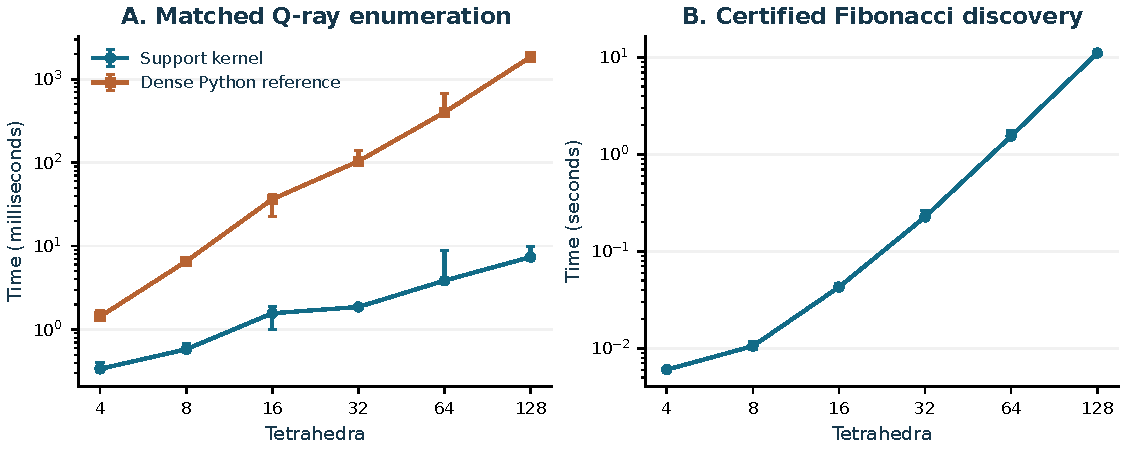
\includegraphics[width=\textwidth]{benchmark_scaling.pdf}
\caption{Measured scaling for two different supplied-sector workloads.
Points are medians; bars span the observed minimum and maximum.
Both axes are logarithmic. The bars describe repeat variability,
not confidence intervals or a distribution over inputs.}
\label{fig:bench}
\end{figure}

The main run completed 176 measured calls and
36 retained warm-up calls on Python 3.12.14.
The frozen runtime and benchmark source hashes were unchanged from the
beginning to the end of that run. A first exploratory timing run is also
retained separately; the tables use only the second, controlled run.
No other agent computation was scheduled concurrently with this main run.


\subsection{What the measurements establish}

The sparse family exhibits the intended removal of triangle-only propagation
from the expensive algebra. The dense Fibonacci family shows that large
support and huge coordinate magnitudes can be handled by the dimension-one
search without sheet expansion. In both cases the measured task remains a
given-sector query.

The corpus also records Regina's default, direct standard double-description,
and via-reduced tree enumeration times, with agreement of their complete
standard vector sets. These are separate reference measurements. Regina's
compiled enumerators are very fast on the small fixtures; our Python code is
not claimed faster than Regina's optimized implementation. Nor do the
measurements establish a speedup in the maintained end-to-end knot pipeline,
which does not yet call this new sector search.

The timing data come from one execution environment and repeated identical
fixtures. They describe these workloads; they are not evidence of a new
unconditional asymptotic bound beyond the proved parameterized results.

\section{Integration, reproducibility, and practical use}
\label{sec:integration}

\subsection{Package layout and dependencies}

The archive contains the complete article source and PDF, the two additive
runtime modules, an unchanged upstream runtime snapshot, deterministic fixture
generators, the frozen independent oracle, audit scripts, all raw results,
focused tests, an integration patch, and source manifests. The runtime search
uses the Python standard library only. Regina 7.4 is needed only to regenerate
the external oracle and its optional reference timing measurements. LaTeX and
Poppler are used for the report build and visual inspection.

The two new modules can be copied into the existing
\path{Topology/UnknotRecognition/fast/fastunknot/} directory. The included
\path{integration.patch} uses repository-relative paths. The existing recognizer
is not modified to treat these supplied-triangulation results as diagram
verdicts. Its normal fallback and its external-backend provenance remain
separate interfaces.

\Needspace{20\baselineskip}
\subsection{Minimal API example}

From the archive root:
\begin{lstlisting}[language=Python]
import sys
sys.path[:0] = ["fast", "scripts"]
from fibonacci_fixture import fibonacci_torus
from fastunknot.normal_sector import discover_in_sector
from fastunknot.normal_sector_verify import verify_sector_witness

fixture = fibonacci_torus(16)
triangulation = fixture["triangulation"]
allowed = [(i, 2) for i in range(16)]
result = discover_in_sector(triangulation, allowed)
assert result["status"] == "DISC_FOUND"
assert verify_sector_witness(triangulation, result["certificate"])
\end{lstlisting}

For a full sector list, use \code{enumerate\_sector} with
\code{phase='standard'} or \code{phase='quadrilateral'}. Standard enumeration
accepts \code{method='auto'}, \code{'arrangement'}, or \code{'supports'}.
The auto method realizes the dispatch in Corollary~\ref{cor:adaptive}.

For bounded outer search:
\begin{lstlisting}[language=Python]
from fastunknot.normal_sector import sparse_disc_search
result = sparse_disc_search(triangulation, max_active=2,
                            max_sectors=1000,
                            max_bases_per_sector=10000)
# Inspect status. A support cutoff is never a knot verdict.
\end{lstlisting}

\subsection{Reproduction commands}

The README gives complete commands with explicit portable paths. The main
entry point runs the frozen-oracle checks without requiring Regina:
\begin{lstlisting}[language=bash]
python3 reproduce.py --quick
python3 reproduce.py --audits
python3 scripts/benchmark.py --large --output results/benchmarks_rerun.json
python3 reproduce.py --build-pdf
\end{lstlisting}
Regenerating the oracle is a separate operation because changing the Regina
version or simplification choices can change the exact triangulation
labelling. The frozen triangulations, their isomorphism signatures, and all
expected vectors are sufficient to rerun the stated comparisons exactly.

\subsection{Limits of the present implementation}

The producer repeatedly prepares geometry when delegating to native component
queries. A trusted immutable prepared-geometry object could reduce that
overhead, but source binding would need to remain explicit. The dense
exhaustion verifier deliberately favors a structurally different computation
over maximum speed. The support search also revisits rays lying in multiple
sectors and has no LP infeasibility cache, dynamic type propagation, or
certified triangulation simplification. These are concrete optimization
opportunities, not assumptions used to justify the current results.

\section{Further research questions and proposed next steps}
\label{sec:future}

\subsection{First priority: reduce choices while retaining dense propagation}

The Fibonacci family shows that large support is sometimes unavoidable, but
its correct sector has one-dimensional matching space. A useful next theorem
should control the number of genuine choices of quadrilateral type, while
allowing long deterministic propagation. Can a partial sector be completed
by exact constraints so that only a small residual set of tetrahedra requires
branching? A complete algorithm would need to prove that its forced choices
are exhaustive and preserve an essential-disc possibility, not merely that
they work on layered examples.

A concrete implementation project is to express forced chains as integer
transfer matrices or short recurrences. One should track the remaining
branching vertices and the bit length of composed maps. The hypothesis
``small residual branching'' must be checked on the actual search path.
It cannot be replaced by the observation that some favorable sequence exists.

\subsection{Second priority: useful negative certificates}

Current complete sector replay reconstructs the ray set. Can absence of a
positive canonical Euler surface be certified by a compact collection of
linear dual witnesses, exploiting the incidence block and the structure of
the minimum-potential function? A single linear Farkas certificate is not
automatically enough for a convex piecewise-linear maximum. A successful
construction must account for every relevant minimum chamber without
encoding an exponentially long list when the output is small.

It is also worth seeking certifiable zero propagation: if exact feasibility
forces a quadrilateral coordinate to vanish, a dual certificate could prune
all descendant sectors sharing that partial assignment.

\subsection{Third priority: certified changes of triangulation}

Sparse-support promises are sensitive to the triangulation. Which elementary
collapses, Pachner moves, layered-solid-torus reductions, or crushing moves
can be applied with bounded encoded cost while preserving a checked
correspondence to the original knot exterior? The desired output is not
just a smaller triangulation; it includes maps sufficient to transfer a
positive witness or a sound negative conclusion.

The main quantitative questions are whether such moves reduce support,
reduce the dimension of useful sectors, or reduce the number of sectors
needed. These objectives need not agree. A move that reduces tetrahedron
count can increase the complexity of a preferred coordinate description.

\subsection{Fourth priority: diagram-to-exterior provenance}

Implement an independently replayable construction of the finite peripheral
triangulation from the diagram, or a checked chain from an already trusted
construction. This would let a successful \code{DISC\_FOUND} become a
source-bound unknot certificate. It would not, by itself, give a fast
negative decision or a quasi-polynomial search bound, but it would connect
the new positive search to the maintained recognizer soundly.

\subsection{Fifth priority: essentiality within a coordinate face}

Under what additional hypotheses does a face containing an essential normal
disc also contain an essential standard vertex disc? The global
Jaco--Tollefson theorem suffices for full search but does not supply this
stronger assertion as stated. Proving an appropriate support-preserving
version would sharpen the parameter in Theorem~\ref{thm:outer} from vertex-disc
support to arbitrary-disc support. A counterexample would be equally useful
because it would identify necessary information for sector pruning.

\subsection{Sixth priority: sharper height and transfer bounds}

The products in Theorem~\ref{thm:height} are often much smaller than $4^k$.
Can one characterize the minors that actually attain large values, replace
column norm four by a graph-dependent product, or exploit a large totally
unimodular submatrix to isolate only a few exceptional quadrilateral columns?
The natural parameter may be the number of columns whose addition genuinely
destroys unimodularity, not the full occupied support.

Any resulting bound should be checked against the exponential-coordinate
layered family. A polynomial coordinate bound in a parameter that remains
constant on that family would be false unless the output uses additional
compressed representation.

\subsection{Seventh priority: reusable source-bound geometry}

The supplied-sector API can cache immutable incidence classes, face equations,
and boundary homology data for repeated queries on the same triangulation.
The independent checker needs either its own cache or an explicit certificate
for the shared object. Cache identity must include the exact source and
algorithm version. Benchmark full queries with fresh and reused preparation,
including A/A controls and certificate replay, before choosing a default.

\subsection{Eighth priority: hierarchy interfaces}

Extend the algebraic sector description to the constrained surfaces used in
hierarchies with boundary patterns. Which additional local normal pieces and
weights preserve the small-column-incidence argument? How large can the
allowed support, cycle rank, boundary pattern, and proof transcript become
after compressed cutting? A local polynomial operation is useful only if
the number and size of interfaces across the hierarchy can also be bounded.
Lackenby's current results provide geometric targets for this work~\cite{lackenby2026}.

\subsection{Ninth priority: careful width-based algorithms}

It is tempting to assume that small treewidth of a dual graph solves the
remaining search. That implication has not been proved here. The exact
positive-Euler normal-surface decision problem parameterized by dual-graph
treewidth was explicitly raised as open in Burton's 2025 Dagstuhl
discussion~\cite{dagstuhl}. A width-based state must preserve unbounded
integer coordinates, compatibility, canonical vertex-link choices, and the
information needed for essentiality. Bounding just the number of graph
boundary vertices is insufficient.

\subsection{Tenth priority: integration benchmarks that measure the objective}

Once diagram provenance and a sector-generation policy exist, run paired
whole-recognition tests against the current pipeline. Include easy knots,
hard unknot diagrams, nontrivial knots with weak polynomial obstructions,
unfavorable sectors, and resource exhaustion. Report failures and overhead,
not only successful disc searches. Until then, fixed-sector query improvements
should continue to be labelled as such.

\section{Research status}

The package proves an exact support kernel and a support-dependent primitive
height bound, implements candidate discovery and independent replay, and
validates the resulting ray sets against a separate topology library. It also
proves a representation-specific obstacle to a uniform sparsity strategy.
The next decisive advance toward the requested quasi-polynomial recognizer
is control of the combinatorial choices of sectors and geometric transitions,
with source-bound provenance. The present contribution provides a concrete,
tested component for that advance while keeping those remaining obligations
visible.

\appendix
\section{Exact source and data provenance}

The archive's \path{results/source_manifest.json} records the GitHub object
identities of 175 retrieved files used for the audit and baseline review.
The runtime snapshot contains only the unchanged Python runtime files needed
for the reproducible package; referenced third-party paper sources are not
redistributed. The two new module hashes appear in every final audit result.
\path{MANIFEST.sha256} checks every delivered file except itself.

The experiment outputs are ordinary JSON with decimal integers. The tested
coordinates are far below Python's default large-decimal-string threshold.
The native upstream certificate integer codec continues to support its
established large-integer encodings. A future public JSON import endpoint
should impose input-size and verification budgets explicitly; this research
package is a local callable API and reproducible command-line workflow.

The separately retained first benchmark run is exploratory. Only the final
source-pinned audit files and the controlled final benchmark provide the
counts and measurements quoted in the main text.

\begin{thebibliography}{99}
\raggedright

\bibitem{tollefson}
J. L. Tollefson,
\emph{Normal surface Q-theory}, Pacific Journal of Mathematics
183(2) (1998), 359--374.
\href{https://doi.org/10.2140/pjm.1998.183.359}{doi:10.2140/pjm.1998.183.359}.

\bibitem{burton2009}
B. A. Burton,
\emph{Converting between quadrilateral and standard solution sets in normal
surface theory}, Algebraic \& Geometric Topology 9(4) (2009), 2121--2174.
\href{https://doi.org/10.2140/agt.2009.9.2121}{doi:10.2140/agt.2009.9.2121}.
\url{https://arxiv.org/abs/0901.2629}.

\bibitem{burton2010}
B. A. Burton,
\emph{Quadrilateral--octagon coordinates for almost normal surfaces},
Experimental Mathematics 19(3) (2010), 285--315.
\href{https://doi.org/10.1080/10586458.2010.10390625}{doi:10.1080/10586458.2010.10390625}.
\url{https://arxiv.org/abs/0904.3041}.

\bibitem{burtonozlen2013}
B. A. Burton and M. Ozlen,
\emph{A tree traversal algorithm for decision problems in knot theory and
3-manifold topology}, Algorithmica 65(4) (2013), 772--801.
\href{https://doi.org/10.1007/s00453-012-9645-3}{doi:10.1007/s00453-012-9645-3}.
\url{https://arxiv.org/abs/1010.6200}.

\bibitem{burtonozlen2014}
B. A. Burton and M. Ozlen,
\emph{A fast branching algorithm for unknot recognition with experimental
polynomial-time behaviour}, arXiv:1211.1079v3, 9 October 2014.
\url{https://arxiv.org/abs/1211.1079v3}.

\bibitem{hlp}
J. Hass, J. C. Lagarias, and N. Pippenger,
\emph{The computational complexity of knot and link problems},
Journal of the ACM 46(2) (1999), 185--211.
\href{https://doi.org/10.1145/301970.301971}{doi:10.1145/301970.301971}.
\url{https://arxiv.org/abs/math/9807016}.

\bibitem{jacotollefson}
W. Jaco and J. L. Tollefson,
\emph{Algorithms for the complete decomposition of a closed 3-manifold},
Illinois Journal of Mathematics 39(3) (1995), 358--406.
The vertex-disc consequence is cited through the explicit statement and
attribution in \cite[Theorem 5.6]{hlp}.

\bibitem{aht}
I. Agol, J. Hass, and W. Thurston,
\emph{The computational complexity of knot genus and spanning area},
Transactions of the American Mathematical Society 358(9) (2006), 3821--3850.
\url{https://arxiv.org/abs/math/0205057}.

\bibitem{burtonbounds}
B. A. Burton, J. Paix\~ao, and J. Spreer,
\emph{Computational topology and normal surfaces: Theoretical and experimental
complexity bounds}, Proceedings of ALENEX 2013, 78--87.
\href{https://doi.org/10.1137/1.9781611972931.7}{doi:10.1137/1.9781611972931.7}.
\url{https://people.smp.uq.edu.au/BenjaminBurton/papers/burton13-bounds-alenex.pdf}.

\bibitem{lackenby2026}
M. Lackenby,
\emph{Incompressible surfaces, hierarchies and unknot recognition},
arXiv:2607.23350v1, 25 July 2026.
\url{https://arxiv.org/abs/2607.23350}.

\bibitem{slides}
M. Lackenby,
\emph{Unknot recognition in quasi-polynomial time},
Oxford lecture slides, March 2021.
\url{https://people.maths.ox.ac.uk/lackenby/quasipolynomial-talk-oxford.pdf}.
The quasi-polynomial announcement is also recorded at
\url{https://www.maths.ox.ac.uk/node/38304}.

\bibitem{regina}
The Regina development team,
\emph{Regina: Software for low-dimensional topology},
version 7.4 used for the independent oracle in this report.
\url{https://regina-normal.github.io/}.

\bibitem{dagstuhl}
M. L\"offler, E. Oh, J. M. Phillips, and A. Weinberger (eds.),
\emph{Computational Geometry (Dagstuhl Seminar 25201)},
Dagstuhl Reports 15(5) (2025), 64--95;
B. Burton's Section 5.2, ``Is Finding Positive Euler Characteristic Normal
Surfaces FPT?''
\href{https://doi.org/10.4230/DagRep.15.5.64}{doi:10.4230/DagRep.15.5.64}.

\end{thebibliography}
\end{document}
